\chapter{Future Work Plan}
\label{chap:future}

In this chapter we break down the the four main objectives we have identified in Chapter \ref{chap:aimsObj} into small working packages, present mile-stones and holidays, relevant conferences, papers we want to publish (either conference or journal). A Gantt-Chart, reflecting all the details is found at the end of this chapter in Figure \ref{fig:gantt}.

\section{The Four Objectives}
\subsection{Functional reactive ABS (FrABS)}
The main goal is to implement a library to be release on Hackage which implements functional reactive ABS (FrABS) using Yampa. As use-cases the Sugarscape- and Agent\_Zero-Model should be implemented. The outcome should be published in a paper (see below) which marks the end of this objective. The time-frame will be until around February 2018.

\subsection{Verification}
The main goal of this objective is to implement our novel idea of verification by refining the EDSL of FrABS to a point where it can be used both as specification- and implementation-language. As use-case we pick the decentralized bilateral bartering as specified in the Sugarscape model. Of central focus will be the research of how to use QuickCheck in the verification process for both the use-case and the FrABS library. The outcome should be published in a paper (see below), summing up the research of this objective.

\subsection{Category Theory view on ABMS}
This is an intermediary objective and serves only for studying basics of category-theory and apply it to ABS to gain a deeper understanding of the deeper structure behind agents, agent-based models and agent-based simulations.  The outcome should be published in a paper (see below), summing up the research of this objective.

\subsection{Validation}
In the final objective we built on all the previous research and combine it into a final paper to show the novel approach to verification and validation using FrABS, QuickCheck and category-theory. Again the use-case will be the decentralized bilateral bartering process as specified in the Sugarscape model but supplemented by theoretical work on bilateral decentralized bartering and real-world examples. Also the category-theoretical view on ABS and on decentralized bilateral trading will be incorporated into this work. The outcome will be a journal-paper to be submitted in the field of ABS (see below).

\section{Planned Papers}
We plan for three papers with at least one of them to be submitted to a journal. This follows the split of the PhD into its objectives: the first concentrates on implementation, the second on verification, the third on category-theory in ABS and the fourth on validation. 

\subsection{FrABS - Towards pure functional programming in ABS}
This paper will present the pure functional approach to ABS we have taken and outlined in Appendix \ref{app:frABS}. It will describe the combination of FRP \& ABS, the EDSL built on top and gives some examples of specification and implementation of the SIRS and Sugarscape model.
For publishing we think of two strategies: either we focus on a conference in the field of ABS or a journal for functional programming. We opt rather for a conference paper, presenting it to an ABS audience because the ABS-community is our intended target - the functional programming people don't have to be convinced that FP is great. Also it is unclear if a functional programming journal accepts the interdisciplinary work (I regard the FP guys to be still open minded but they may be rather conservative compared to ABS community?). The target-journal/conference is yet to be determined.

\subsection{Verification in pure functional ABS}
In this paper we will discuss the verification method we have developed using our FrABS implementation and QuickCheck. We describe the decentralized bilateral bartering process of the Sugarscape model and verify it.
We may come to the conclusion to collapse this paper into the fourth, validation paper if it is better suited there. In any case a paper will be written (I am constantly writing down insights, results and explanations during the process of research, so writing up the paper in the end is only about restructuring and cleaning-up) whether it will be published or not is not that important - it will definitely go into the final thesis.

\subsection{Category-Theory in ABMS}
In this paper we will present our research about a category-theoretical view on ABS. 
We may come to the conclusion to collapse this paper into the fourth, validation paper if it is better suited there. In any case a paper will be written (I am constantly writing down insights, results and explanations during the process of research, so writing up the paper in the end is only about restructuring and cleaning-up) whether it will be published or not is not that important - it will definitely go into the final thesis.

\subsection{Validation in pure functional ABS}
This paper will present our novel approach to validation in ABS using our FrABS library and category-theory. We will validate the decentralized bilateral bartering process as specified in the Sugarscape model against theoretical models and real-world examples. This paper is definitely intended to be a journal-paper because of its central importance to the PhD, its original novelty and the range and depth of the content. The target-journal is yet to be determined but we want to focus primarily on an agent-based modelling journal.

\section{Years Overview}

\subsection{1st Year}
In the first year, all is about orientation, experimenting and finding out what the PhD is \textit{really} going to be about. In the remaining time the goal is to finalize the FrABS library and to release it on Hackage. We will start studying category-theory to build up knowledge to be used in the 3rd year.

\subsection{2nd Year}
In the second year, the focus will be on \textit{verification}. Using the FrABS library and QuickCheck we will research how far we can go into formalizing model-specifications and how well we can do verification. The second focus we will be on continuing studying category-theory to gain a deep-enough understanding to use it for validation in the 3rd year.

\subsection{3rd Year}
In the third year I will look into \textit{validation} with category-theory, focus on cleaning up the research and writing the final thesis. The plan is to start the writing of the final thesis around April 2019 with a 5-months writing-window and to submit on-time at end of September 2019.

\section{Conferences}
\begin{itemize}
	\item \textbf{Multi-Agent Systems AAMS} - General Multi-Agent Systems and Agent-Based Modelling \& Simulation, Deadline in November
	\item \textbf{Social Simulation Conference SSC} - New Methods and models in simulation, Deadline in March
	\item \textbf{Symposium on Trends in Functional Programming} - Functional programming stuff, Deadline in May
\end{itemize}

\section{Mile-Stones}
\begin{itemize}
	\item 2017 31st March - finished and submit Paper 
	\item 2017 18th June - Finished writing 1st year report 
	\item 2017 3rd July - Oral annual report
	\item 2017 October - 2nd year starts
	\item 2018 May - Submit Paper on FrABS
	\item 2018 October - 3rd year starts
	\item 2019 February - Submit Paper on Verification
	\item 2019 April - Begin of thesis-writing
	\item 2019 September - Submit Thesis
	\item 2019 30th September - official end of PhD
	\item 2020 30th September - end of pending-period
\end{itemize}


\label{app:gantt}
\begin{landscape}
	\begin{figure}
		\label{fig:gantt}
  		\caption{Gantt-Chart for remaining PhD}
  		\centering
  		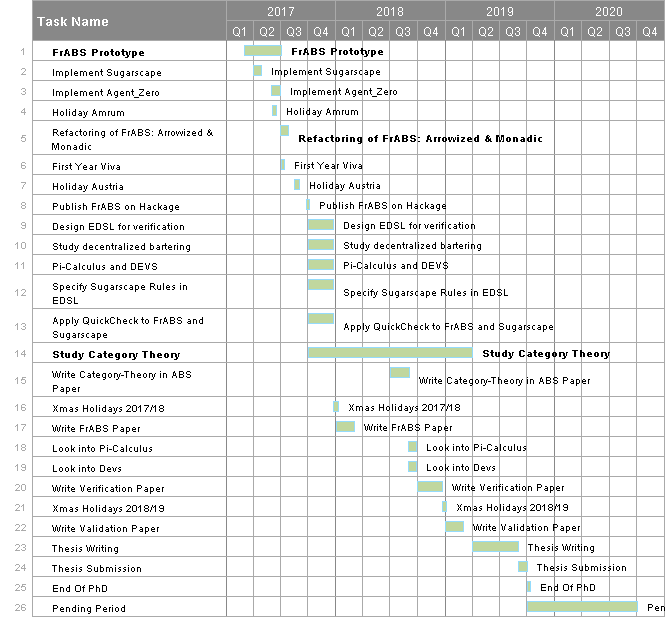
\includegraphics[width=1.2\textwidth]{./charts/gantt.png}
	\end{figure}
\end{landscape}